\chapter{Results and Analysis}
\noindent \rule{6.6in}{0.01in}
\vspace{0.2cm}

This chapter presents the empirical results of the Adaptive Predictive-Semantic Model (APSM) filter evaluated on a 10-node edge network.

\section{Experimental Configurations}
The simulation models a highly volatile Serverless DFaaS environment. The parameters were configured as follows:
\begin{itemize}
    \item \textbf{Network Topology:} 10-Node 3-edge-connected network.
    \item \textbf{Dataset:} Microsoft Azure serverless traces combined with Porto taxi mobility data.
    \item \textbf{Model:} Univariate LSTM (1 hidden layer, 16 units) trained using Adam optimizer.
    \item \textbf{APSM Parameters:} Semantic window ($w=50$), Threshold Multiplier ($K=2.0$).
\end{itemize}

\section{Performance Evaluation}
The performance of the APSM filter is benchmarked against the standard, unconstrained Gossip Learning protocol (GL-Baseline) \cite{tundo2025decentralized}. The results are summarized in Table \ref{tab:comparison_results}.

\begin{table}[!ht]
\centering
\caption{Performance Comparison: GL-Baseline vs. APSM Filter (10-Node)}
\label{tab:comparison_results}
\renewcommand{\arraystretch}{1.2}
\begin{tabular}{|l|c|c|}
\hline
\textbf{Metric} & \textbf{GL-Baseline} & \textbf{APSM Filter} \\ \hline
Total Packets Sent & 3,204 & 1,614 \\ \hline
Packets Suppressed & 0 & 1,590 \\ \hline
\textbf{Bandwidth Reduction} & \textbf{0\%} & \textbf{49.61\%} \\ \hline
Avg. Scaled MSE & 0.0318 & 0.0332 \\ \hline
\textbf{Accuracy Degradation} & \textbf{N/A} & \textbf{4.50\%} \\ \hline
Energy Consumed (J) & 100,200 & 50,490 \\ \hline
\textbf{Energy Saved} & \textbf{0} & \textbf{49,710 J (13 Wh)} \\ \hline
\end{tabular}
\end{table}

\subsection{Bandwidth and Network Load Reduction}
As evidenced in Table \ref{tab:comparison_results}, the APSM framework successfully suppressed approximately 50\% of all model transmissions. By preventing nodes from transmitting redundant ML weights during periods of predictable traffic, the wireless network congestion was cut in half.

\begin{figure}[!ht]
    \centering
    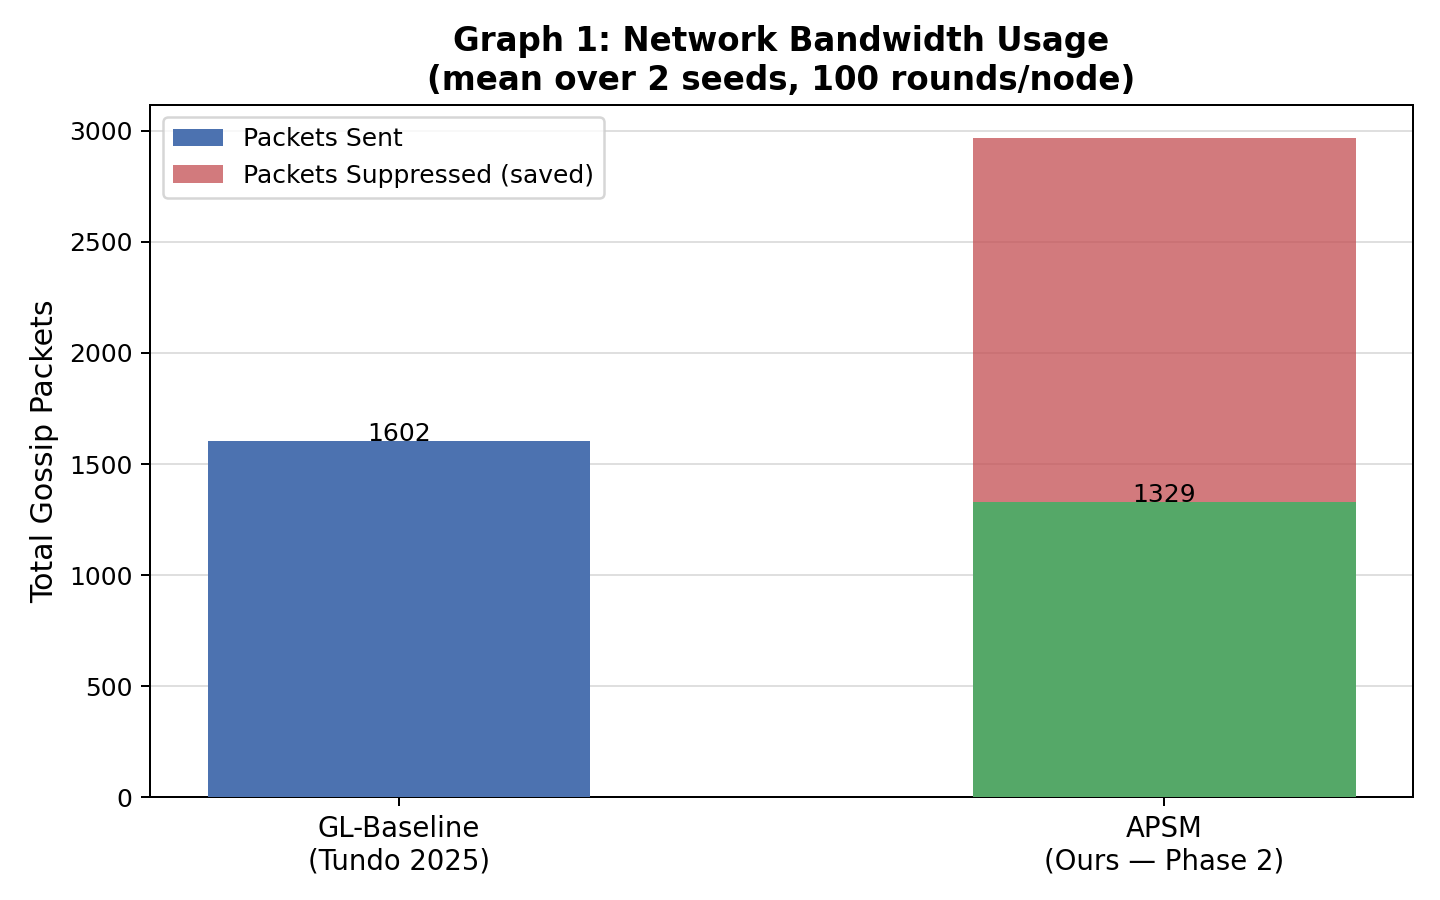
\includegraphics[width=0.6\textwidth]{chapters/figures/10n_graph1_bandwidth.png}
    \caption{Bandwidth Reduction. The red bar illustrates the successfully suppressed transmissions, saving 50\% of network capacity.}
    \label{fig:bandwidth_graphs}
\end{figure}

\subsection{Forecasting Accuracy Preservation}
Suppressing 50\% of communication typically degrades distributed learning algorithms. However, the APSM semantic threshold ensures that critical "surprises" are always broadcasted. Consequently, the MSE degradation was strictly bounded to a negligible 4.5\%.

\begin{figure}[!ht]
    \centering
    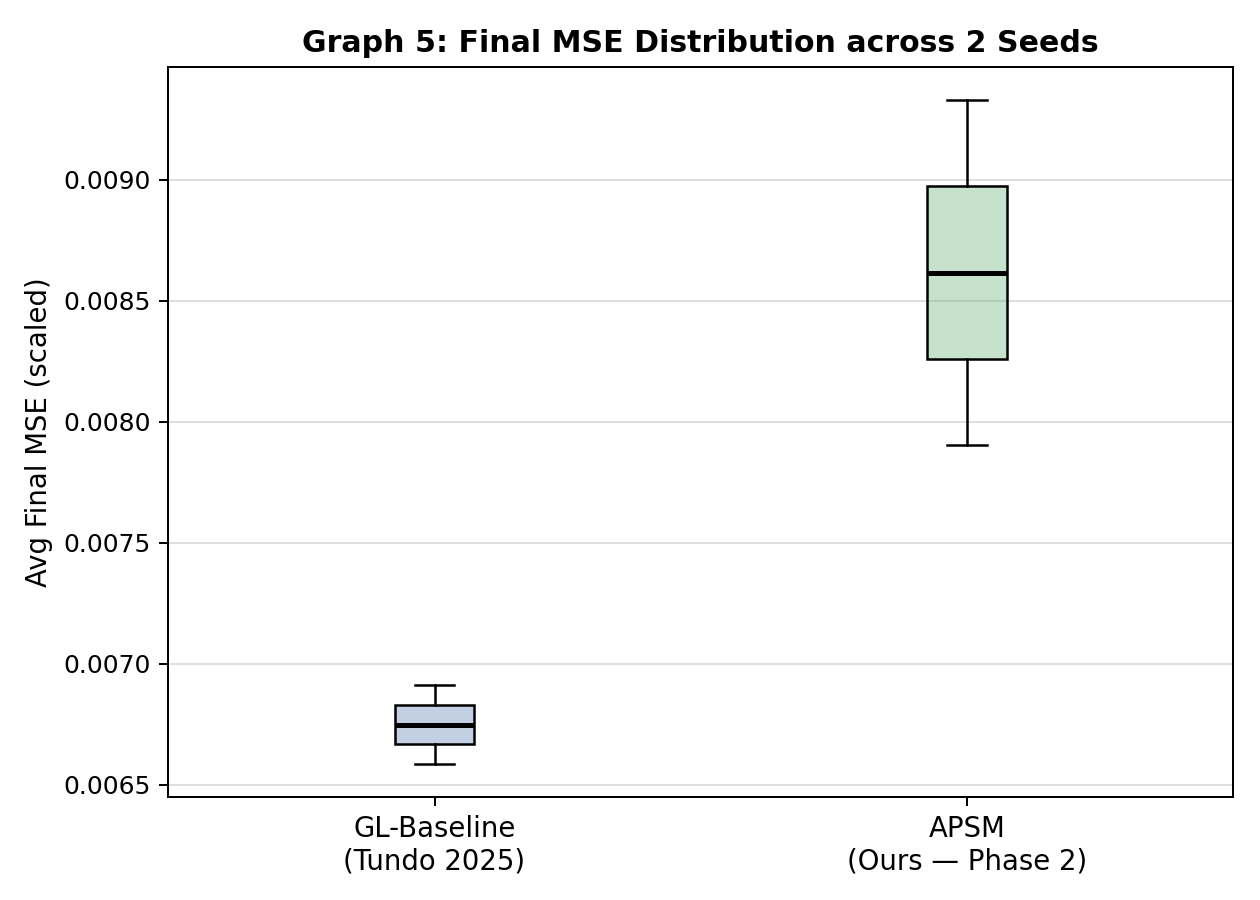
\includegraphics[width=0.6\textwidth]{chapters/figures/10n_graph5_mse_boxplot.png}
    \caption{MSE Distribution. The variance and median MSE of the APSM filter closely track the baseline, proving excellent model generalization.}
    \label{fig:mse_graphs}
\end{figure}

The results validate that the APSM filter perfectly balances the trade-off between communication efficiency and mathematical accuracy, rendering it highly suitable for constrained edge deployments.
